Image reconstruction is required to produce images of activity distribution from the acquired tomographic measurements. The methods of that process can be separated in two categories, analytical methods and statistical or iterative methods.  
Analytical reconstruction methods make use of linear analytic approaches based on analytical formulations of the acquisition and reconstruction process to estimate an image. These methods treat the measured LOR data as line integrals over image space and necessitate corrections to be applied on projection data prior of reconstruction, in order to result to valid and quantitatively accurate images. The most commonly used and fastest analytical reconstruction method is the Filtered Back Projection which is covered briefly in this chapter. 
Statistical reconstruction treat the reconstruction problem as a non-linear problem that require iterative optimisation methods to reach a solution. The aim of iterative reconstruction is to reach a solution that best explain the tomographic data, by incorporating a model of the imaging system and accurate modeling of the noise in the raw data from the detection process. This approach is generic and allow for multiple effects , including corrections, to be accounted for in the system model as well as additional prior information about the image or the dynamic processes in the data. These are the main reasons for which iterative reconstruction is nowadays the standard reconstruction in clinical PET and it is the reconstruction process used in this thesis due to its ability to incorporate complex system models and dynamic models. 

\subsection{Projection and back-projection process}
Coincidence detection of annihilation photons in PET leads naturally to a line-integral model where the number of coincidence events is an \gls{lor} is approximately linearly proportional to the integral of tracer density along the volume joining the two detectors. 
In the simplified case of a 2D image space and a single ring 2D PET scanner, the projection process can be written as:

\begin{equation}
   \bm y = proj\{\bm{\lambda}\}  \\, 
  \label{eqn:Radon}
\end{equation}

where $\bm{\lambda}$ is the continuous distribution of radiotracer in the imaging system's FOV and $\bm{y}$ the projection data (or else sinogram data). 

The projection operation is also known as the Radon transform~\cite{radon1917} and translates the data from the image to the projection domain. The inverse operation that translates from data space to image space is back-projection.

The radiotracer distribution is modelled using a set of spatial basis functions that described the distribution as a set of parameters. The use of equally sized non-overlapping voxels is commonly chosen, or alternatively use of overlapping spheres (blobs)~\cite{Matej1996}. Here we consider voxels, which result in a discrete representation of the radiotracer distribution $\lambda_j$, with $j=1..n_j$ being the voxel index. 
Equivalently the projection space is discretised based on the \glspl{lor} defined by the detectors as $y_i$ , with $i=1..n_m$ the projection bin index.

Projection and back-projection can be treated by summing contributions of voxels to each projection bin. Different projector methods exist that model the contribution of voxels differently depending on their placement in the \gls{lor}. The short list that follows list some commonly used methods that can also be used in CASToR. 

\begin{itemize}
\item  Siddon projector~\cite{Siddon1985}: Weights the contribution of an LOR to each by the length of the line that intersects the voxel.
\item  Distance driven~\cite{DeMan2004}: An optimised method for calculating weights by mapping pixel boundaries and detector boundaries for each projection to a common axis .
\item  Incremental Siddon~\cite{Jacobs2015}.
\item  Joseph~\cite{Joseph1982}: Estimates contribution of voxels to LOR based on linear interpolation and their distance from the LOR. 
\item  Multi-Siddon~\cite{Moehrs2008}: Uses multiple lines from the faces of the detectors in each LOR to approximate the volume intersected between the two detectors and the voxel.
\end{itemize}

\begin{figure} [h!]
\centering
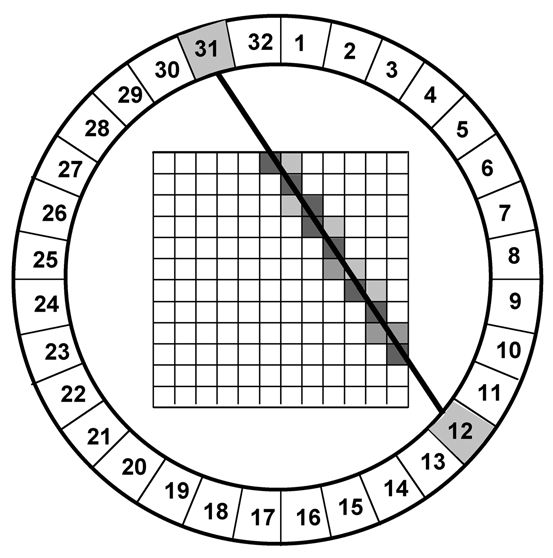
\includegraphics[scale=0.35,angle=0]{2_Theory_Methods/figures/Radon_Discrete.png}
\caption{Back-projection of a single LOR through image space, with contribution weighted according to the length of the line that intersects the voxel.} 
\label{fig_3:back_projection.}
\end{figure} 

The analytical reconstruction method of filtered back projection estimates the image though the process of back-projecting all the data in image space where the contributions from all LORs are superimposed. In practice a filtered version of the projections is back-projected to account for the non-uniform number of contributions from LORs in image space, which gives the name of filtered back projection to this analytical reconstruction method. The method can be extended to 3D via use of the 3D X-ray transform and approximations of missing data projections~\cite{Kinahan1989}. 

But while analytical reconstruction are linear processes that produce estimates relatively fast, accuracy is limited by the assumptions of the line integral model , positron range effects, variations in response across an LOR etc. Finally these methods do not account for the statistical properties of the data. They assume noise-free data and equal weighting between LORs, which for noisy data results to image artefacts that require post reconstruction smoothing to be reduced. 


\subsection{Statistical formulation of the problem \& iterative reconstruction}
One main advantage of iterative reconstruction methods is the ability to make use of complex models that map the radiotracer distribution from image space to data space, which can include physical processes such as positron range effects, scatter, random contributions, attenuation effects etc. The ability to accurately model the detection process leads to improvements in image resolution. The second most important advantage of iterative reconstruction methods is the inherent accounting for the statistical variations in the detection process via the use of a probabilistic model. Some of the disadvantages of these methods is that they are computationally more demanding, although this is a lesser problem with continuing advancements in computing technology. Another disadvantage is that these methods are non linear and could result in unpredictable behaviour under certain conditions and when terminated before convergence (which is commonly the case in practice, where early termination is used to limit the induction of image noise). 

\subsubsection{system model and statistical model}
The detection system is modelled as a linear process that maps the activity distribution $\bm\lambda$ to the data $\bm{y}$ though a projection or system matrix $\bm{P}$. 

We will assume that: 
\begin{itemize}
\begin{small}
\item $\lambda_j^{(k)}$: static image intensity for voxel $j$ of $n_j$ voxels, at iteration $k$
\item $y_i$: number of events for bin $i$
\item $\bm{y}$: event data \{$y_i, i=1,...,n_i$\}
\item $d $: decay factor
\item $\Delta t$: Duration of acquired data
\item $X_{ij}$: geometrical projector 
\item $ A_i$: attenuation factor
\item $N_i$: efficiency factor
\item $r_i, s_i$: rate of scattered and random coincidences
\item $R_i, S_i$: Total scattered and random coincidences
\end{small}
\end{itemize}

Given an initial guess of the image $\bm\lambda^{(k)}$ , the model of the mean or expectation of the data can be written as

\begin{equation}
   \bm\hat{y_i} = \sum_j X_{ij} \lambda_j^{(k)} + R_i + S_i  = \sum_j X_{ij} \lambda_j^{(k)} + r_i\Delta t + s_i\Delta t  \\.
  \label{eqn:model_mean)}
\end{equation}

As the detection of annihilation photons can be modelled by a Bernoulli process, the number of counts in each projection bin will be a sample from a Poisson distribution. According to the Poisson probability model, the conditional probability or likelihood function for $\hat{y_i}$ given the measured data ${y_i}$ will be

\begin{equation}
p({y_i}|{\hat{y_i}}) = L({\hat{y_i}}|{y_i}) = e^{-{y_i}} \frac{\hat{y_i}^{y_i}}{{y_i}!}  \\ \\  , 
\label{eqn:bin_likelihood)}
\end{equation}

and under the assumption that measurements of counts in each bin are independent random processes the likelihood can be expanded for all the data

\begin{equation}
p(\bm{y}|\bm{\hat{y}}) = L(\bm{\hat{y}}|\bm{y}) = \prod_i e^{-\hat{y_i}} \frac{\hat{y_i}^{y_i}}{{y_i}!} \\ \\ .
\label{eqn:likelihood)}
\end{equation}

In this process we seek to find an image estimate  $\bm\lambda^{(k)}$ that maximises the likelihood. Equation~\ref{log_likelihood} can be written more simply as the log likelihood

\begin{equation}
    lnL(\bm{\hat{y}}|\bm{y})  = \sum_i  -\hat{y_i} + y_i ln(\hat{y_i}) - ln({y_i}!)  \\ ,
    \label{eqn:log_likelihood)}
\end{equation}since the ln function is monotonic, maximising the log likelihood function in equation~\ref{eqn:log_likelihood)} is equivalent in maximising likelihood equation~\ref{eqn:likelihood)}. By including the system model, the problem can be expressed as: 

\begin{equation}
    lnL(\bm{\lambda}|\bm{y})  = \sum_i\left[  -\sum_j (X_{ij} \lambda_j + R_i + S_i) + y_i ln(\sum_j X_{ij} \lambda_j + R_i + S_i) - ln({y_i}!) \right]
\end{equation}

This expression serves as the cost function for the iterative reconstruction process, which we seek to optimise. 


\subsubsection{Optimization}

For simplicity in the derivation process we temporarily will ignore the additive corrections from the system model, and the log-likelihood function is:

\begin{equation}
    lnL(\bm{\lambda}|\bm{y})  = \sum_i\left[  -\sum_j (X_{ij} \lambda_j) + y_i ln(\sum_j X_{ij} \lambda_j) - ln({y_i}!) \right]
    \label{eqn:simpleloglikelihood}
\end{equation}

The optimization seeks to find an image $\bm\hat\lambda$ distribution that maximises the log-likelihood function.

\begin{equation}
\bm\hat\lambda = \argmax{\bm{\lambda}}lnL(\bm{\lambda}|\bm{y})
\end{equation}













